During the early stages of the project we began searching for existing solutions to draw inspiration to the design and implementation phases. All members of the group have previously had experience using different recipe sites on the Internet, and we  think that the existing solutions lack functionality. We will in this section review and discuss the existing solutions and draw some good practices from these.  

\section{Supercook}
Supercook\cite{supercook} is a website with focus on searching for recipes by their ingredients. The user is limited to enter a set of ingredients which is defined by Supercook. When adding ingredients to a search the user is aided by autocompletion and a word cloud with ingredients. The word cloud changes according to the type of ingredients you have entered, e.g. if you enter ``vanilla'' the word cloud will change to contain typical cake ingredients. It is possible to apply restrictions to your search, e.g. ``I don't eat meat''. A search on Supercook will result in a prioritised list of links to recipes from several online cookbooks. A screenshot of the website is shown in Figure \ref{fig:supercook}.

By evaluating the search results of Supercook we have deduced what we believe are the steps used to generate the search results:
\begin{enumerate}
	\item Remove recipes without matching ingredients.
	\item Sort by most matching ingredients.
	\item Sort by least missing ingredients.
\end{enumerate}
We have also noticed some quirks in the way it counts matching ingredients. It seems like the search algorithm counts the number of occurrences of the entered ingredients in the recipes. When entering ``bell pepper'' and ``olive oil'', recipes which contain both red, green, and yellow pepper are prioritised higher than recipes which actually contains both of the entered ingredients. It also appear as if ingredients in the recipes are mapped to the recipes defined by Supercook. An example of that is that ``flour'' appear to be mapped to ``flour'', ``wheat'', ``oat'', etc. This also appear to have the shortcoming that recipes containing e.g. ``wheat flour'' are prioritised as if they have two matching ingredient when the user entered ``flour''.

When making a search containing ``eggs'', ``garlic'', ``ground beef'', and ``onion'', we get a result which showcases a drawback of the sorting done by Supercook. The first 94 recipes are simple recipes using only few of the entered ingredients, including 24 recipes on how to boil an egg. Recipe number 95 is a recipe for meatballs and is using all entered ingredients but it also needs ``bread crumbs''. The reason why the first 94 recipes are prioritised highest is because they do not need any other ingredients than the ingredients entered.
\begin{figure}[H]
\centering
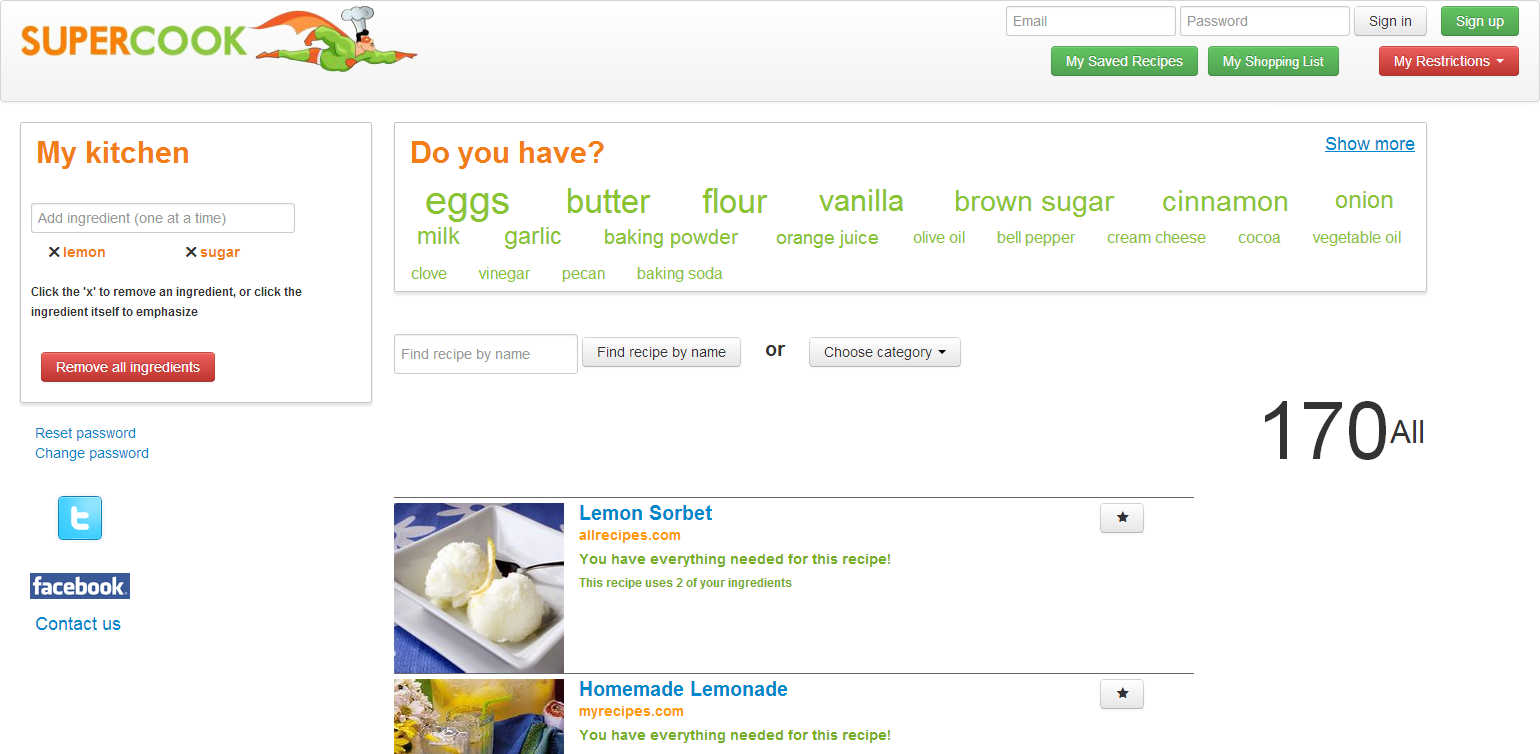
\includegraphics[width=\linewidth]{img/screenshots/supercook.png}
\caption{The inferface of Supercook.}
\label{fig:supercook}
\end{figure}

\section{Allthecooks}
Allthecooks is one of the most downloaded \cite{allthecooks-googleplay} Android applications that is related to the search: ``recipe''. The application has a great design that follows the Android guidelines\cite{guidelines-appstructure} which makes it is intuitive and easy to navigate. The detailed display of a recipe is especially well implemented, the user has everything on a single activity, and can easily see the needed ingredients and the required steps to cook the recipe. The user can also by a press of a button toggle between different measuring units, or add the selected ingredient to a shopping list. Screenshots of the application is shown in Figure \ref{fig:allthecooks-menu}, \ref{fig:allthecooks-detail1}, \ref{fig:allthecooks-detail2}, and \ref{fig:allthecooks-detail3}. 
The recipes of Allthecooks are user created, meaning they are created and uploaded by users. The photos are also provided by users, this can be dangerous if the photos are not checked for content not suitable for the application's audience. The good thing about user created recipes are that the application is growing with the audience of the application.
The search is free-text based, which means that opposite the Supercook web application it is hard to find recipes based on ingredients. You are able to apply filters to your search to remove recipes that certain ingredients.
\twofigs{screenshots/menu.png}{Menu of Allthecooks}{fig:allthecooks-menu}{screenshots/rainbowcake-1.png}{Detail display of a recipe}{fig:allthecooks-detail1}
\twofigs{screenshots/rainbowcake-2.png}{Buttons for different features}{fig:allthecooks-detail2}{screenshots/rainbowcake-3.png}{Directions for the recipe}{fig:allthecooks-detail3}

\section{BigOven}
BigOven is also one of the most downloaded \cite{bigoven-googleplay} Android application that is related to ``recipe''. The application's navigation and design does not follow the Android guidelines\cite{guidelines-appstructure} and therefore the application's navigation can be quite confusing to an Android user.
The application main page is cluttered and presents the user with many functionalities, see \autoref{fig:mainpage-bigoven}. It would be better to implement a navigation drawer and separate each function to its own view. 
It is possible to make an ingredient search and recipe search. The ingredient search is limited to only three ingredients and the algorithm finds only the recipes were they all are included, The ingredient search is based on free-text, meaning the user does not have the aid of autocompletion, like Supercook. If the user inputs three ingredients that have no real relation like; ``beef'', ``cake-mix'', ``salmon'', the ingredient search would find no results, the ingredient search excludes everything that does not contain all three ingredients.
Like Allthecooks the user can add the different ingredients to a shopping list, save the recipe to favourites, and alternate between the metric and imperial system.
A cool feature that is unique to the BigOven application is the Menu-Cards, see \autoref{fig:menucards-bigoven}.
\twofigs{screenshots/mainpage-bigoven.png}{The main page of BigOven}{fig:mainpage-bigoven}{screenshots/menucards-bigoven.png}{Menu Cards from BigOven}{fig:menucards-bigoven}
It is a small collection of different recipes that together builds to a meal, e.g. ``steak'', ``fries'', and ``green beans''. Each meal is bound to a day, which means that the user can create a Menu-Card that can contain a meal for each day of the week, or more.
The recipes of BigOven is also like Allthecooks user created, which provides the same risks and benefits as explained in the previous section.
The BigOven application is free, but you can buy Pro-features that exclude advertisers from the application and unlocks more functionality in the application.

\section{Comparison}
After a small preview of the already existing solutions, of both web and android applications. We believe that we can create an application with improved features, such as a better search algorithms, easy navigation, and an elegant design. We like the idea of being able to search for recipes by ingredients, but we wont exclude the possibility to also search directly for recipes. We will also provide the user with different input styles; text-type-input(free text for recipe search and ingredient restricted), and tile-input. Tile input is basically the same as ingredient restricted input, but instead of typing the name of each ingredient the user selects the ingredient by use of tiles. The ingredient are divided into categories and maybe even subcategories, to make the navigation more sensible, otherwise the user would be presented with a too many tiles and the screen would be cluttered.

\begin{table}[H]
\centering
\begin{tabular}{|l|l|l|l|}
\hline
 & \textbf{Supercook} & \textbf{Allthecooks} & \textbf{BigOven} \\
\hline
\textbf{Platform} & Website & Android/Website & Android/Website \\
\hline
\textbf{Cost} & Free & Free & Free \& Paid \\
\hline
\textbf{Recipe search} & No & Yes & Yes  \\
\hline
\textbf{Ingredient search} & Yes & No & Yes \\
\hline
\textbf{Recipe origin} & Web crawl & User defined & User defined \\
\hline
\textbf{Shopping list} & Yes & Yes & Yes \\
\hline
\textbf{Menu planner} & No & Yes & Yes \\
\hline
\textbf{Saving recipes} & Yes & Yes & Yes \\
\hline
\textbf{Ingredient filter} & Yes & Yes & Yes \\
\hline
\textbf{Sharing of shopping list} & No & E-mail/SMS & E-mail \\
\hline
\textbf{Sharing of recipe} & No & App/SMS/E-mail & App/E-mail \\
\hline
\end{tabular}
\caption{Application comparison}
\label{tab:appcomparison}
\end{table}

